\subsection{Versuchsaufbau}
\label{sec:Versuchsaufbau}
\begin{figure}
	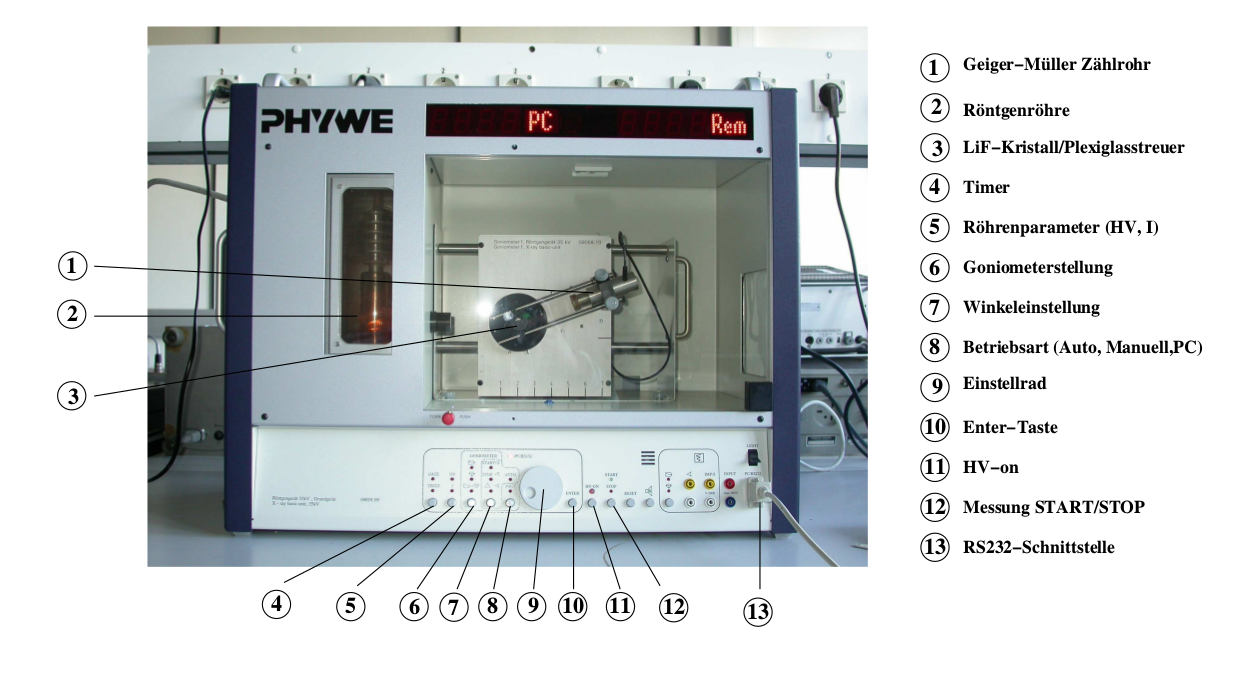
\includegraphics[width=1.0\textwidth]{nIKO_und_jULIAN_ÜLADS/aufbau.png}
	\caption{Aufbau der Versuchsapparatur. \cite{Anleitung}}
	\label{fig:aufbau}
\end{figure}

Der Versuchsaufbau ist in Abbildung \ref{fig:aufbau} dargestellt.
Dabei sind die wichtigsten Bestandteile die Kupfer-Röntgenröhre, ein Lithiumfluorid-Kristall
und das Geiger-Müller-Zählrohr.
Das Röntgengerät ist mit einem Rechner verbunden und kann mithilfe des Programms "Measure"
bedient werden.
Hier lässt sich der Kristallwinkel und der Drehmodus festlegen.
Die Beschleunigungsspannung wird auf $U_{\mathrm{B}}=\SI{35}{\kilo\volt}$ eingestellt.
Es ist darauf zu achten, dass die Schlitzöffnung am Geiger-Müller-Zählrohr waagerecht
ausgerichtet ist, damit nur ein Winkel gemessen wird und kein ganzes Spektrum.
Bei den Messungen für die Untersuchung der Absorptionsspektren können die jeweiligen Absorber
vor dem Geiger-Müller-Zählrohr angebracht werden.
